Gedurende de handshake van TLS wordt door de client een lijst van ondersteunde cipher suites aangeboden aan de server. De server selecteert daaruit de door de server meest gewenste suite en communiceert dat terug naar de client. Hiermee ligt vast welke cipher suite er gebruikt gaat worden.

Zowel de client als de server hebben dus invloed op welke cipher suite gebruikt gaat worden. Het is belangrijk om zo'n sterk mogelijke cipher suite te kiezen. Als je echter alleen de sterkste cipher suites in je browser toestaat dan kan het gebeuren dat je niet meer bij sommige sites kan komen omdat deze die suite niet ondersteunt, het omgekeerde kan natuurlijk ook, dat je als server alleen de sterkste suites ondersteunt en dat sommige browsers je site niet kunnen bezoeken omdat ze die suite niet ondersteunen. Security is altijd een afweging tussen sterke beveiliging en voldoende gebruiksvriendelijkheid.

Om te bepalen welke cipher suites je wel en niet wil toestaan is er een site die voor je bijhoudt welke suites geschikt zijn en welke je absoluut niet meer moet gebruiken omdat ze te makkelijk te kraken zijn. Deze site is te vinden op \url{https://ciphersuite.info/cs/?singlepage=true&security=secure}. Door de optie security=secure mee te geven zie je alleen de suites die een kwalificatie secure of hoger hebben.

Via je browser kan je opvragen welke suite er gekozen is voor een bepaalde site. Door op het slotje in de adresbalk van je browser te klikken en te kiezen voor meer informatie krijg je bij Firefox een overzicht te zien zoals in figuur \ref{fig:CipherAIVD} is te zien.

\begin{figure}[htbp]
	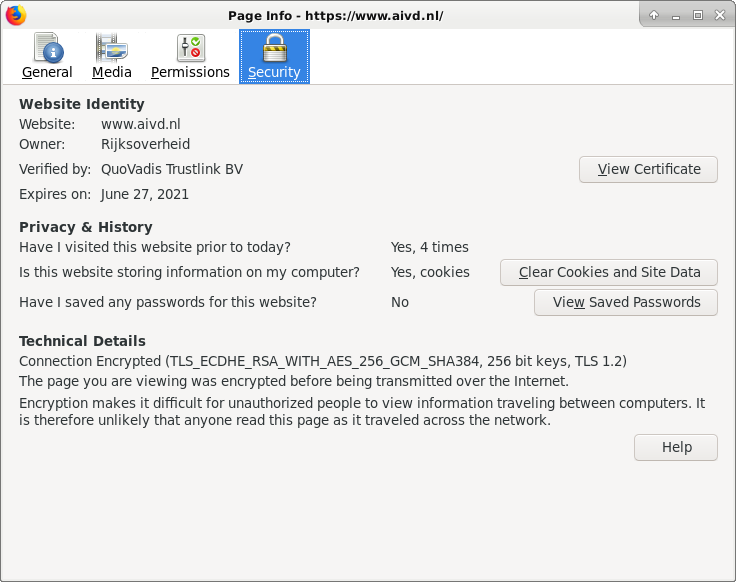
\includegraphics[width=0.9\linewidth]{security_ciphers_aivd.png}
	\caption{Cipher Suite van de AIVD}
	\label{fig:CipherAIVD}
\end{figure}

Bij Technical Details vind je de regel die gaat over de connectie encryptie. Je ziet dat er gekozen is voor TLS 1.2 en 256 bits en dat de cipher suite TLS\_ECHDE\_RSA\_WITH\_AES\_256\_GCM\_SHA384 is. Dat is een hele mondvol, de vraag is wat dit betekent.

\goodbreak
\begin{description}
	\item[TLS] Het TLS protocol waarvan we aan het einde van de regel al gezien hebben dat de keuze gevallen is op TLS versie 1.2
	\item[ECDHE] Het key exchange protocol, Elliptic-Curve Diffie-Hellman Ephemeral.
	\item[RSA] Het encryptie protocol voor de certificaten. De client moet dus RSA gebruiken om de public key te decrypten.
	\item[AES\_256\_GCM] De symmetrische encryptie methode die gebruikt gaat worden voor de encryptie. Alle berichten tussen client en server worden dus versleuteld met 256 bits AES encryptie met Galois/Counter Mode.
	\item[SHA384] Message integrity. Om te controleren dat berichten onderweg niet zijn gewijzigd wordt de SHA functie gebruikt in 384 bits mode.
\end{description}

Het TLS protocol wordt gebruikt (en niet bijvoorbeeld SSL), we gebruiken een vorm van Diffie-Hellman om een symmetrische encryptie sleutel overeen te komen en deze sleutel gebruiken we met AES om alle berichten te encrypten en decrypten. Daarnaast hebben ze besloten om RSA te gebruiken voor de public en private key en worden de berichten gecontroleerd door gebruik te maken van de SHA-hashing techniek. Daarmee hebben we de volledige cipher suite beschreven.
